\documentclass{article}
\usepackage[normalem]{ulem}
\usepackage[utf8]{inputenc}
\usepackage{graphicx}
\usepackage{mathtools}
\usepackage{amssymb}
\usepackage{amsmath}
\usepackage{macros}
\usepackage{color}
\newcommand{\Or}{{\mathcal{O}}}

\begin{document}
  \section{Taylorutvecklingar, elementära Maclaurinutvecklingar}
  % img 1
  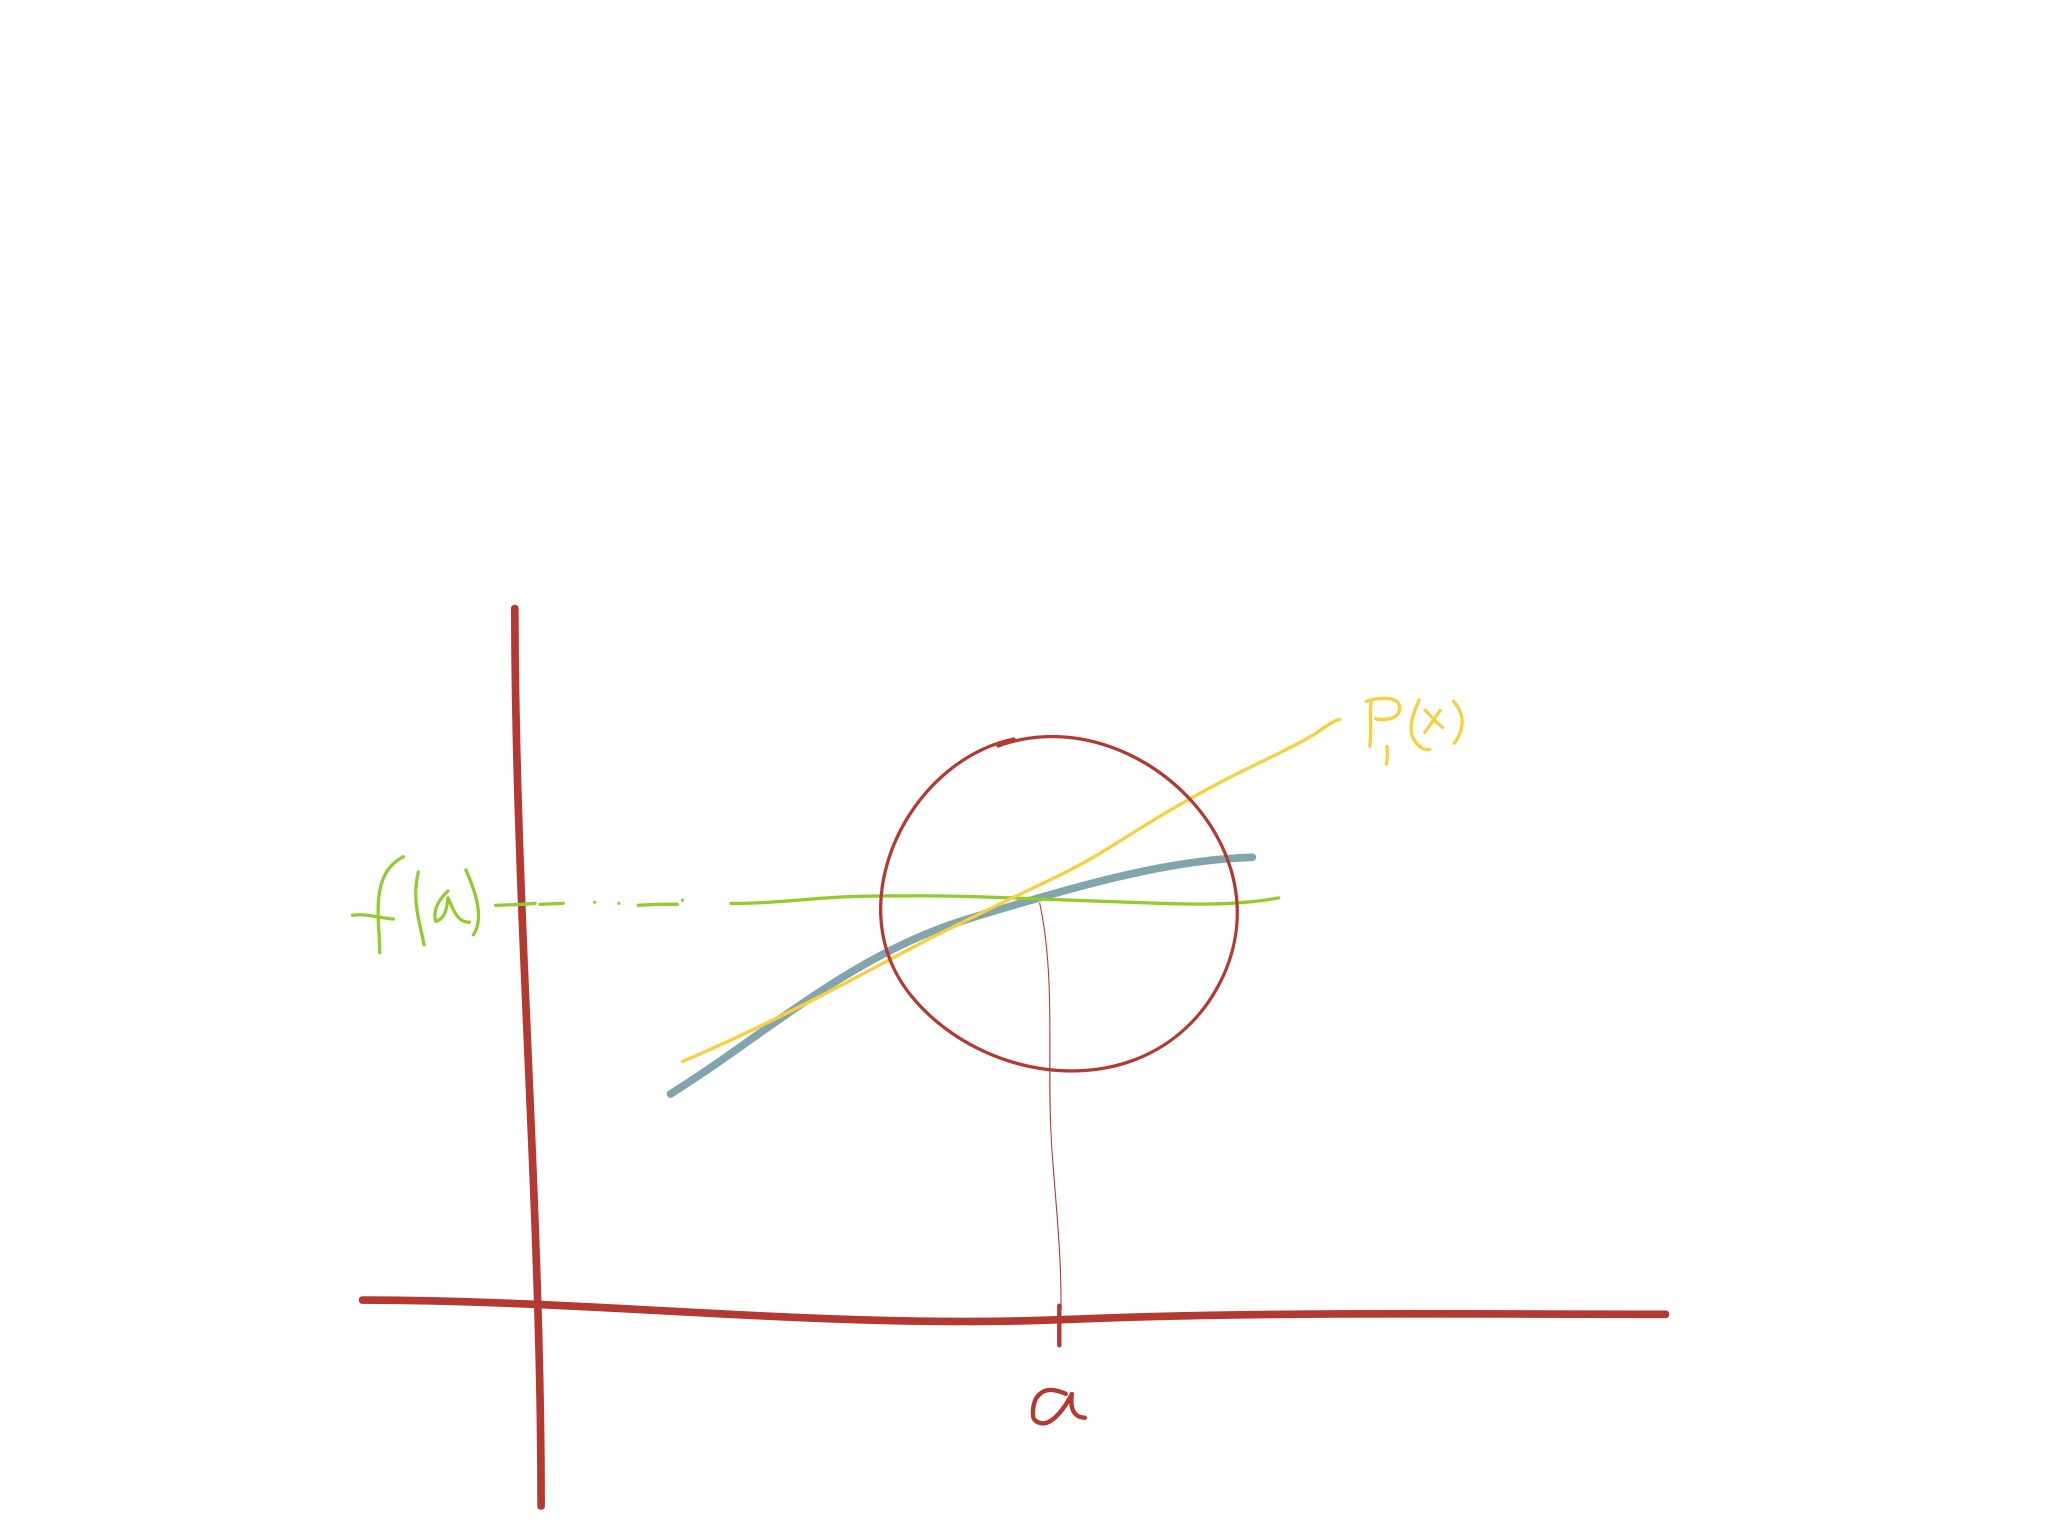
\includegraphics[scale=0.20]{img/img1.jpg}
  $$ p_0(x) = f(a), f \text{ är kontinuerlig } \im f(x)-p_0(x)\to 0, x\to a  $$
  $$ p_1(x) = f(a)+f'(a)(x-a), f, f' \text{ är kontinuerliga } \im f(x) - p_1(x) \to 0, x\to a $$
  $$ p_1(a) = f(a), p'_1(a)=f'(a) $$
  $$ p_n(x) =
  \begin{cases}
    p_n(a)=f(a)\\
    p'_n(a)=f'(a)\\
    \hdots\\
    p_n^{(n)}(a)=f^{(n)}(a)
  \end{cases}
  $$
  Taylorpolynom av ordning n:
  $$ p_n(x) = f(a) + f'(a)(x-a) + \f{f''(a)}2(x-a)^2+\dots+\f{f^{n}(a)}{n!}(x-a)^n$$
  Taylorutveckling av ordning n:
  $$ f(x) = f(a) + f'(a)(x-a) + \f{f''(a)}2(x-a)^2+\dots+\f{f^{n}(a)}{n!}(x-a)^n + r(x)$$

  \section{Ex. 1}
  Bestäm Taylorutvecklingar av ordning 3 av $f(x)=\ln x$ kring $a=1$.
  $$ f(x) = f(1) + f'(1)(x-1) + \f{f''(1)}2 (x-1)^2+\f{f'''(a)}{3!}(x-1)^3 + r(x)$$

  $$
  \begin{cases}
    f(x) = \ln x \im f(1) = 0\\
    f'(x) = \f 1x \im f'(1) = 1\\
    f''(x) = -\f 1{x^2} \im f''(1) = -1\\
    f'''(x) = \f 2{x^3} \im f'''(1) = 2
  \end{cases}
  $$

  $$ \ln x = 1(x-1) - \f 12 (x-1)^2 + \f 2{3!}(x-1)^3 + r(x) \eq $$
  $$ \ln x = (x-1) - \f 12 (x-1)^2 + \f 13(x-1)^3 + r(x) $$


  \section{Restterm i ordo form}
  $$ r(x) = \Or((x-a)^{n+1}) \eq r(x) = b(x)(x-a)^{n+1} $$
  Där $b(x)$ är en begränsad funktion dvs $ \abs{b(x)} \le C $\\
  % img 2
  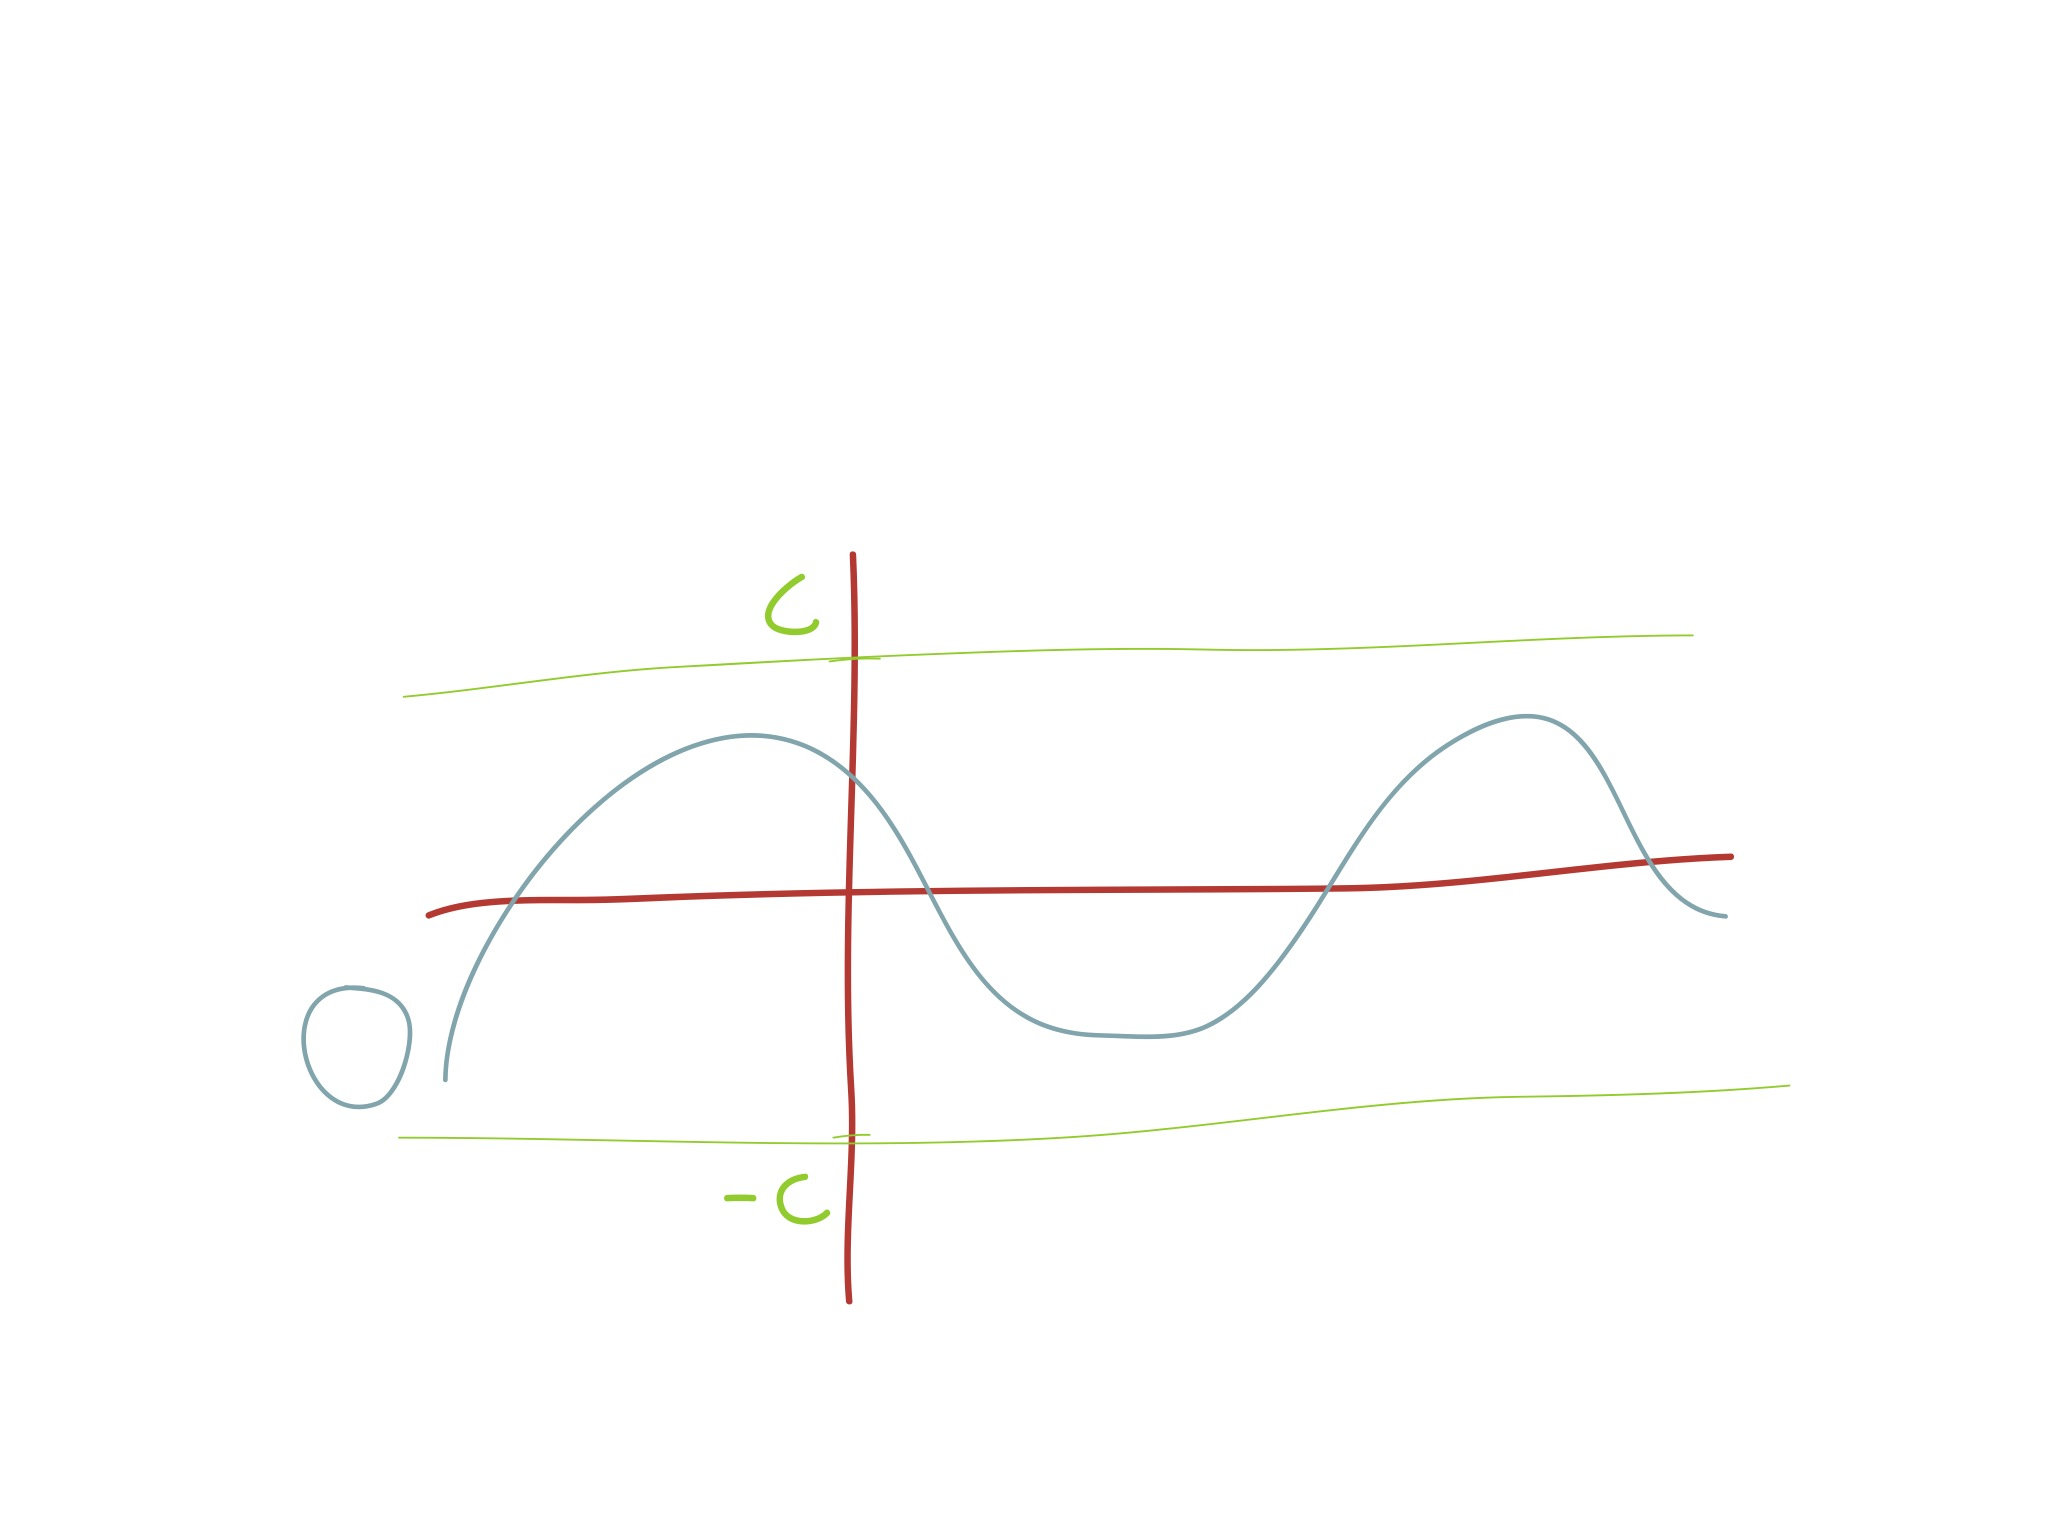
\includegraphics[scale=0.20]{img/img2.jpg}\\

  \section{Sats}
  Om $f$ har kontinuerliga derivator upp till och med ordning n i $[\alpha, \beta]$ och $a\in [\alpha, \beta]$ så:
  $$ f(x) = f(a) + f'(a)(x-a) + \f{f''(a)}2(x-a)^2+\dots+\f{f^{n}(a)}{n!}(x-a)^n + \Or((x-a)^{n+1})$$

  $$a=0\im$$
  Maclaurinpolynom av ordning n:
  $$ f(x) = f(0) + f'(0)x + \f{f''(0)}2x^2+\dots+\f{f^{n}(0)}{n!}x^n$$
  $$ f(x) = f(0) + f'(0)x + \f{f''(0)}2x^2+\dots+\f{f^{n}(0)}{n!}x^n + \Or(x^{n+1})$$

  \section{Ex. 2}
  Bestäm Maclaurinutveckling av ordning 3 av $f(x)=e^x$
  $$ f(x) = f(0) + f'(0)x + \f{f''(0)}2x^2+\f{f^{3}(0)}{n!}x^3 + \Or(x^4)$$
  $$ f(x) = f'(x) = f''(x) f'''(x) = e^x$$
  $$ e^x=1+x+\f 12 x^2 + \f 1{3!}x^3 + \Or(x^4) $$
  Antag att $ \abs{x}<0.1 \im \abs{r(x)} = \abs{b(x)x^4}= \abs{b(x)}\abs{x^4} \le C 0.1^4 = C 10^{-4}  $

  \section{Ex. 3}
  Bestäm Maclaurinutveckling av ordning 3 av $f(x)=\cos x$
  $$
  \begin{cases}
    f(x) = \cos x \im f(0) = 1\\
    f'(x) = -\sin x \im f'(0) = 0\\
    f''(x) = -\cos x \im f''(0) = -1\\
    f'''(x) = \sin x \im f'''(0) = 0
  \end{cases}
  $$
  $$ \cos x = 1 - \f 12 x^2 + \Or(x^4) $$

  \section{Räkning med stort ordo}
  % img 3
  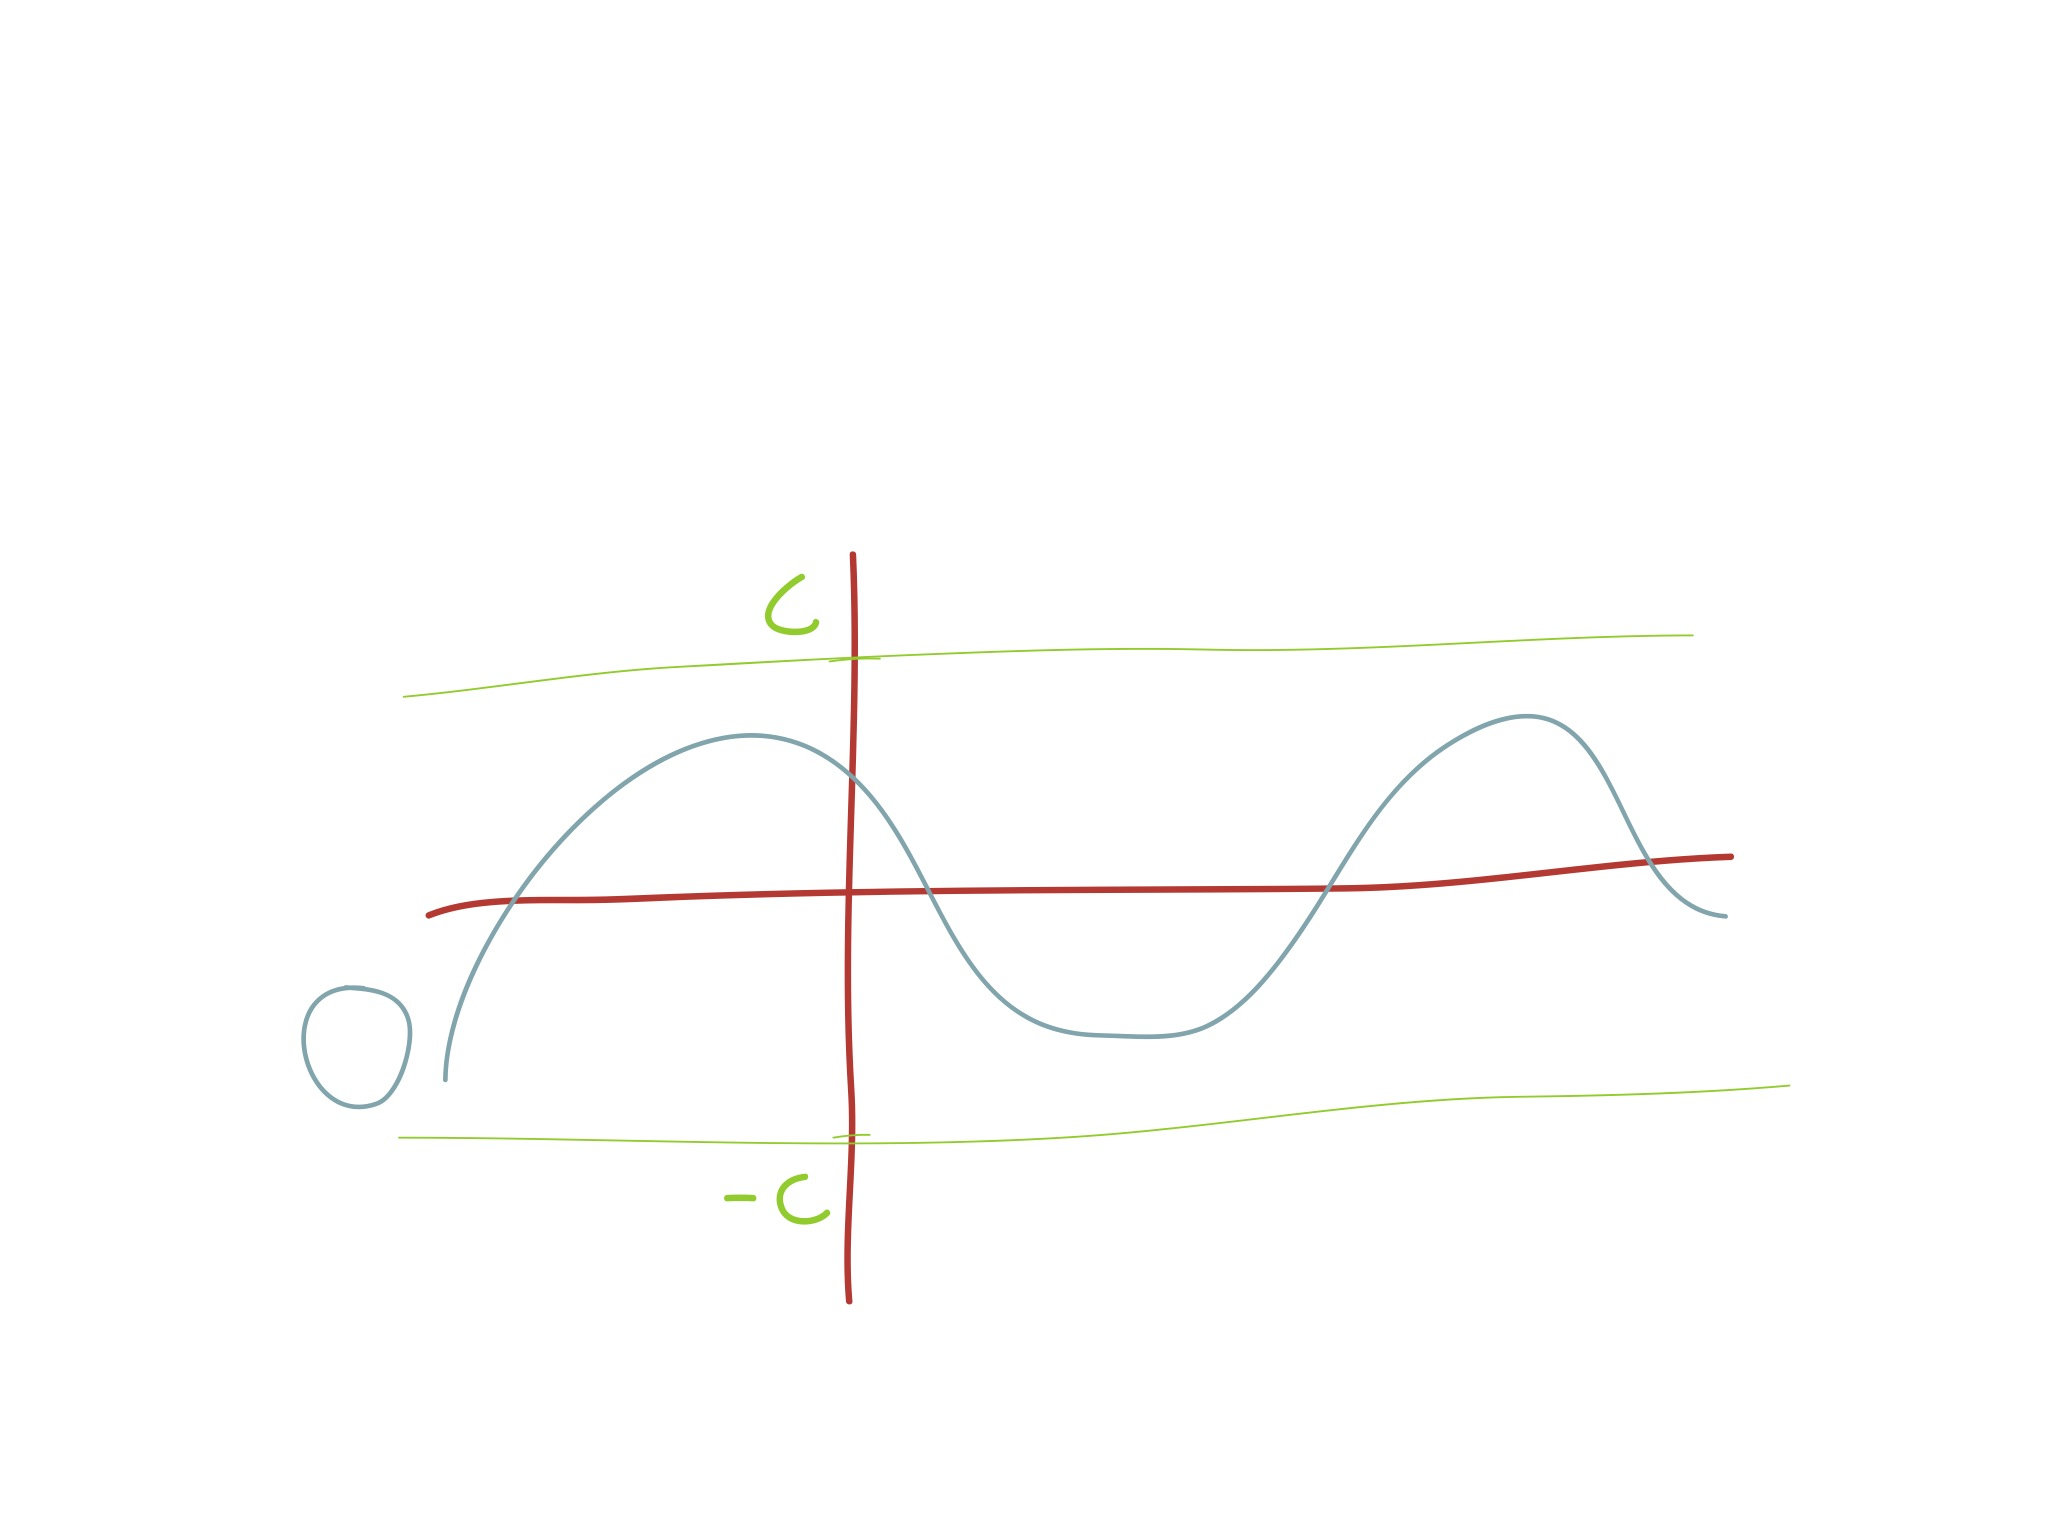
\includegraphics[scale=0.20]{img/img2.jpg}\\
  $ r(x) = \Or(x^n) \eq r(x) = b(x) x^n, $ där $ \abs{b(x)} \le C $ nära 0
  \begin{enumerate}
    \item $\Or(x^n) \Or(x^m) = \Or(x^{n+m})$\\
      k är konstant $\im k \Or(x^m) = \Or(x^m)$
    \item $\Or(x^n)+\Or(x^m) = \Or(x^n)$ om $n\le m$\\
      Obs! $\Or(x^n) - \Or(x^n) = \Or(x^n)$
  \end{enumerate}
  \subsection{Bevis}
  \begin{enumerate}
    \item $\Or(x^n) \Or(x^m) = \pa{b_1(x)x^n}\pa{b_2(x)x^m} = \pa{b_1(x)b_2(x)}x^{n+m} = \Or(x^{n+m})$\\
      $x^n \Or(x^m) = \Or(x^n+m)$
    \item $\Or(x^n) + O(x^m) = \pa{b_1(x)x^n}+\pa{b_2(x)x^m} = x^n(b_1(x) + b_2(x)x^{m-n}) = \Or(x^n), n\le m $\\
      $\Or(x^n) - \Or(x^n) = b_1(x)x^n - b_2(x)x^n = (b_1(x)-b_2(x))x^n = \Or(x^n)$
  \end{enumerate}

  \subsection{Standard Maclaurinutvecklingar}
  $$ e^{x} = \sum^{\infty}_{n=0} \frac{x^n}{n!} = 1 + x + \frac{x^2}{2!} + \frac{x^3}{3!} + \cdots\quad\text{ for all } x\! $$
  $$ \sin x = \sum^{\infty}_{n=0} \frac{(-1)^n}{(2n+1)!} x^{2n+1} = x - \frac{x^3}{3!} + \frac{x^5}{5!} - \cdots\quad\text{ for all } x\! $$
  $$ \cos x = \sum^{\infty}_{n=0} \frac{(-1)^n}{(2n)!} x^{2n} = 1 - \frac{x^2}{2!} + \frac{x^4}{4!} - \cdots\quad\text{ for all } x\! $$
  $$ \ln(1+x) = \sum^\infty_{n=1} (-1)^{n+1}\frac{x^n}n\quad\text{ for } |x| < 1 $$
  $$ (1+x)^\alpha = \sum_{n=0}^\infty {\alpha \choose n} x^n\quad\text{ for all }|x| < 1 \text{ and all complex } \alpha\! $$
  $$ \arctan x = \sum^{\infty}_{n=0} \frac{(-1)^n}{2n+1} x^{2n+1}\quad\text{ for }|x| \le 1, x\not=\pm i\! $$

  \section{Ex. 4}
  $$ \lim_{x \to 0} \f{1-\cos x}{x \sin x} = \bmat{ \sin x = x+\Or(x^3)\\ x\sin x = x\pa{x+\Or(x^3)}\\ = x^2 + \Or(x^4) } = \lim_{x\to 0} \f{1-\pa{1-\f {x^2}2 + \Or(x^4) }}{x^2 + \Or(x^4)} =$$
  $$ \lim_{x\to 0} \f{\f {x^2}2 + \Or(x^4)}{x^2 + \Or(x^4)} = \lim_{x\to 0} \f{x^2\pa{\f 12 + \Or(x^2)}}{x^2\pa{1+\Or{x^2}}} = \lim_{x\to 0} \f {\f 12 + \Or(x^2)}{1+\Or(x^2)} = \f 12 $$

  \section{Ex. 5}
  Bestäm Maclaurinutveckling av ordning 9 av $f(x)=\sin(x^2)$
  $$ f(t) = \sin t $$
  $$
  \begin{cases}
    f(x) = \sin t \im f(0) = 0\\
    f'(x) = \cos t \im f'(0) = 1\\
    f''(x) = -\sin t \im f''(0) = 0\\
    f'''(x) = \cos t \im f'''(0) = -1\\
    f^{(4)}(x) = \sin t \im f^{(4)}(0) = 0\\
    \dots
  \end{cases}
  $$
  $$ \sin t = t - \f {t^3}{3!} + \Or(t^5) = \bra{t=x^2} = \sin(x^2) = x^2 - \f {x^6}{3!} + \Or(x^{10})$$

  \section{Sats (entydlighet av Maclaurinutveckling)}
  Om
  $$ f(x) = c_0 + c_1 + c_2x^2 + \dots + c_nx^n + \Or(x^{n+1}) $$
  Där $ c_0, c_1, \dots, c_n $ är konstanter.\\
  Då är detta Maclaurinutvecklingen av ordning n.\\

\end{document}
